\documentclass{../bredelebeamer}
\usepackage{multirow}
\usepackage{pdfpages}
\usepackage{braket,bigstrut}
\usepackage{palatino}
\usepackage{multicol,bigstrut}
\usepackage{listings}
\usepackage{tikz}
\usepackage{tikz-3dplot}
\usepackage{pgfplots}
\pgfplotsset{compat=1.17}
\usepackage{booktabs}
\usepackage{amsmath,amssymb,amsfonts,cancel,physics,siunitx}
\usepackage{enumitem}
\setlist[itemize]{leftmargin=1.03em, label={$\bullet$}}
\usepackage[outline]{contour} % glow around text
\contourlength{0.9pt}
\usetikzlibrary{positioning,shadows,backgrounds,calc,bending}%

% Define custom TikZ styles for detector diagram (from template.sty)
\colorlet{veccol}{green!50!black}
\colorlet{myred}{red!70!black}
\colorlet{myblue}{blue!70!black}
\colorlet{mydarkred}{red!40!black}
\colorlet{mydarkblue}{blue!30!black}
\colorlet{CMScol}{red!80!black}
\colorlet{ATLAScol}{blue!80!black}
\definecolor{miverde}{RGB}{44,162,67}
\definecolor{azulF}{rgb}{.0,.0,.3}
\tikzset{>=latex}
\tikzstyle{axis}=[->,thick,line cap=round]
\def\ang{19} % angle for detector rotation
\tikzstyle{detector}=[thick,draw=mydarkred,rotate around z=\ang]
\tikzstyle{beam pipe}=[draw=blue!20!black!50,fill=blue!20!black!10,rotate around z=\ang]
\tikzstyle{detector surface}=[red!60!black!60,opacity=0.06,rotate around z=\ang]

\setbeamercolor{footnote mark}{fg=black}
\setbeamercolor{footnote}{fg=black}
\usepackage{appendixnumberbeamer}

% Define custom colors for better readability
\definecolor{SignalOrange}{RGB}{255,140,0}
\definecolor{EfficiencyRed}{RGB}{220,20,60}
\definecolor{WeightPurple}{RGB}{148,0,211}
\definecolor{SysGreen}{RGB}{34,139,34}
\definecolor{LumiBlue}{RGB}{0,71,171}

\renewcommand{\baselinestretch}{0.9}

\usepackage[backend=bibtex8,style=authortitle,autocite=footnote]{biblatex}
\addbibresource{referencia.bib}

\renewbibmacro*{cite:title}{%
	\printtext[bibhyperref]{%
		\printfield[citetitle]{labeltitle}%
		\setunit{\space}%
		\printtext[parens]{\printdate}%
	}%
}
\renewcommand{\figurename}{{\bf Fig.}}
\usefonttheme{serif} % default family is serif

% Define arXiv command for stylized formatting
\newcommand{\arxiv}{ar$\chi$iv:}

\renewcommand{\baselinestretch}{0.9}

\title[Final Dissertation]{Machine Learning-Enhanced Feasibility Studies on the Production of New Particles with Preferential Couplings to Third Generation Fermions at the LHC}
\subtitle{}
\author[ML-BSM3G@LHC - C. Rodríguez]{%
    \vspace{2em}\\
    PhD(c). Cristian Fernando Rodríguez Cruz\inst{1}\\
    \href{mailto:c.rodriguez45@uniandes.edu.co}{c.rodriguez45@uniandes.edu.co}\\
    \vspace{1em}
    Research advisors:\\
    \vspace{0.5em}
    Prof. Andrés Florez\inst{1} ( \href{mailto:ca.florez@uniandes.edu.co}{ca.florez@uniandes.edu.co} )\\
    \vspace{0.5em}
    Prof. J. Jones-Pérez\inst{2} ( \href{mailto:jones.j@pucp.edu.pe}{jones.j@pucp.edu.pe} )\\
    \vspace{1em}
}

\institute[]{\inst{1} Universidad de los Andes\and
\inst{2} Pontificia Universidad Católica del Perú
}
\date{\today}
\lstset{language=C++,
  basicstyle=\ttfamily,
  keywordstyle=\color{blue}\ttfamily,
  stringstyle=\color{red}\ttfamily,
  commentstyle=\color{green}\ttfamily,
  morecomment=[l][\color{magenta}]{\#}
}

\newcounter{finalframe}

% Flag to control section divider frames
\newif\ifsectiondividers
\sectiondividersfalse  % Set to false to hide divider frames
\sectiondividerstrue   


\begin{document}
\frame{\titlepage}

\begin{frame}
    \frametitle{Outline}
    \tableofcontents
\end{frame}

\section{Introduction}

\ifsectiondividers
\begin{frame}
\centering
\vfill
{\Huge \textbf{Introduction}}
\begin{center}
		\includegraphics[width=1\linewidth]{../Images/intro.png}
\end{center}
\end{frame}
\fi

\subsection{Standard Model of Particle Physics}
\begin{frame}{Standard Model of Particle Physics: A Successful Framework}
	\begin{minipage}[t]{0.39\textwidth}
        \begin{block}{Core Theoretical Structure}
            \begin{itemize}[leftmargin=1.03em, label={$\bullet$}]
                \item \textbf{Fermion Sector:} 
                \begin{itemize}[leftmargin=0.803em, label={$\circ$}, itemsep=0.2em]\footnotesize
					\item 3 generations
                    \item Left-handed doublets:
                    $$
					  Q_L = \begin{pmatrix}
						q_{u} \\ q_{d}
					  \end{pmatrix}_L; 
					  \quad
					  L_L = \begin{pmatrix}
						\ell \\
						\nu_{\ell}
					  \end{pmatrix}_L
					$$
					\item Right-handed singlets: $q_{uR}, q_{dR}$; $\ell_R$
                    \item Flavor structure from  CKM mixing
                    \item Initially, $\nu_R$ not required (no mass)
                \end{itemize}

				\vspace{0.5em}
                \item \textbf{Gauge Group:} 
                \begin{itemize}[leftmargin=0.803em, label={$\circ$}, itemsep=0.2em]\footnotesize
					\item $SU(3)_C \times SU(2)_L \times U(1)_Y$
                    \item Strong force: $SU(3)_C$ (QCD)
                    \item Electroweak: $SU(2)_L \times U(1)_Y$
                \end{itemize}
                
                \vspace{0.5em}
                \item \textbf{Higgs Mechanism:}
                \begin{itemize}[leftmargin=0.803em, label={$\circ$}, itemsep=0.2em]\footnotesize
                    \item $SU(2)_L \times U(1)_Y \to U(1)_{\text{EM}}$
                    \item Masses to $W^\pm$, $Z^0$ bosons 
					\item Massless $\gamma$
                    \item Fermion masses via Yukawa couplings
                    \item Higgs boson $h$ discovered (LHC 2012)
                \end{itemize}
            \end{itemize}
        \end{block}
    \end{minipage}
	\hfill
    \begin{minipage}[t]{0.58\textwidth}
        $ $ \vspace{0.4em}
        \centering
        \includegraphics[width=\textwidth]{../Images/SM.png}
        
        \vspace{0.3em}
        \begin{block}{Key Features}
            \begin{itemize}\footnotesize
                \item \textbf{Particle spectrum:} 12 fermions + 5 bosons
                \item \textbf{QFT:} Renormalizable, gauge invariant, anomaly-free
                \item \textbf{Tested experimentally:} Exceptional agreement with data
                \item \textbf{Predictive power:} Successfully tested at LHC
            \end{itemize}
        \end{block}
    \end{minipage}

\end{frame}

\subsection{Deficiencies of the SM}
\begin{frame}{Deficiencies of the SM}
    \begin{minipage}[t]{0.43\linewidth}
        \begin{block}{The SM cannot be complete:}
            \begin{itemize}
                \item Unexplained $\nu$ masses
                \item No explanation for DM
                \item Matter-antimatter asymmetry \\unsolved
                \item Gravity not included
            \end{itemize}
        \end{block}

        \vspace{0.5em}

            \includegraphics[width=.9\linewidth]{../Images/SM-2.png}
    \end{minipage}
    \hfill
    \pause
    \begin{minipage}[t]{0.53\linewidth}
        \textbf{Experimental hints of New Physics:}
    
        \vspace{0.3em}
        \makebox[\linewidth][l]{\hspace*{-0.8cm}\includegraphics[width=1.25\linewidth]{../Images/rdrds_ckm2025_new.pdf}}

		\vspace{0.5em}
        Recent measurements of the $R(D)$ and $R(D^*)$ ratios show a $\sim 3\sigma$ deviation from SM predictions, suggesting possible lepton universality violation.

    \end{minipage}
\end{frame}

\begin{frame}{B-Meson Anomalies}
	\begin{minipage}{0.48\textwidth}
		\begin{block}{$R_{K}$ Anomalies}
			\begin{equation*}
				R_{K} = \frac{\mathcal{B}(B \to K \mu^+ \mu^-)}{\mathcal{B}(B \to K e^+ e^-)}
			\end{equation*}
			\begin{center}
				\includegraphics[width=\linewidth]{../Images/rk_anomalie.png}
			\end{center}
		\end{block}
	\end{minipage}
	\hfill
    \begin{minipage}{0.48\textwidth}
		\begin{block}{$R_{D}$ Anomalies}
			\begin{equation*}
				R_{D} = \frac{\mathcal{B}(B \to D \tau \nu)}{\mathcal{B}(B \to D \ell \nu)}
			\end{equation*}
			\begin{center}
				\includegraphics[width=\linewidth]{../Images/rd_anomalie.png}
			\end{center}
		\end{block}
	\end{minipage}
	{\large
		\begin{itemize}
			\item The B-meson anomalies hint at lepton flavor universality violation.
			\item NP coupled mainly to 3G-fermions address these anomalies.
			\item Currently, $R_K$ is SM-compatible, tensions in $R_D$ still persist.
		\end{itemize}
	}
\end{frame}

\subsection{LHC and Beyond the SM Physics}
\begin{frame}{The Large Hadron Collider (LHC)}
	\begin{minipage}{.59\textwidth}
		\begin{center}
		\includegraphics[width=\linewidth]{../Images/LHC.png}
	\end{center}
	\begin{block}{LHC Physics Program}
		\begin{itemize}
			\item SM parameter determinations
			\item Precision Tests
			\item Direct searches for BSM physics
			\item Cross sections \& Decay rates measurements
			\item Angular Correlations, among others
		\end{itemize}
	\end{block}
	\end{minipage}
	\hfill
	\begin{minipage}{.38\textwidth}
		\begin{block}{World's largest particle collider:}
		%\vspace{-1.2em}
			\begin{itemize}
				\item Located at CERN, at the France-Switzerland border
				\item 27 km circumference ring
				\item Designed to probe the TeV scale
				\item Four main experiments: \\ATLAS, CMS, LHCb, ALICE
				\item pp collisions at $\sqrt{s} = 13.6$ TeV
				\item Bunches of $\sim10^{11}$ Particles
				\item 40 MHz collision rate
				\item Small beam spot size
				\item Run-II Luminosity $\sim 150 \text{ fb}^{-1}$
				\item RUN-III currently on analysis \\with $\sim 300 \text{ fb}^{-1}$
				\item High luminosity upgrade \\(HL-LHC) planned for 2029
			\end{itemize}
	\end{block}
	\end{minipage}
	
\end{frame}


\begin{frame}{Collider Observables}
	\begin{minipage}{.45\textwidth}
		\begin{block}{Collider Kinematics}
			$
			\begin{cases}
				\text{Pseudorapidity: } \eta = -\ln\tan(\theta/2) \\
				\text{Transverse momentum: } p_T = p \sin(\theta) \\
				\text{Azimuthal angle: } \phi\\
				\text{Deposited energy: } E \\
			\end{cases}
			$
		\end{block}
	\end{minipage}
	\hfill
	\begin{minipage}{.50\textwidth}
		\begin{center}
        \includegraphics[width=0.90\linewidth]{../Images/real_event.png}
    \end{center}
	\end{minipage}

	\begin{center}
		\scalebox{0.8}{		% CMS detector - left perspective
		\tdplotsetmaincoords{75}{50} % to reset previous setting
		\begin{tikzpicture}[scale=2.6,tdplot_main_coords,rotate around x=90]
			
			% VARIABLES
			\def\rvec{\L/2/cos(\thetavec)}
			\def\thetavec{18}
			\def\phivec{60}
			\def\L{3.3}    % detector length
			\def\R{0.75}   % detector cylinder radius
			\def\l{4.3}    % beam pipe length
			\def\r{0.04}   % beam pipe radius
			\def\rt{0.042} % beam pipe radius + line thickness
			\def\xmax{1}   % maximum x axis
			\def\ymax{1}   % maximum y axis
			\def\zmin{-\l/2-0.2} % minimum z axis
			\def\zmax{\l/2+0.3}  % maximum z axis
			\def\w{0.3}
			\coordinate (O) at (0,0,0);
			\coordinate (Z) at (0,0,\L/2);
			\tdplotsetcoord{O'}{0.022}{\thetavec}{\phivec} % slightly shifted origin
			\tdplotsetcoord{O''}{0.018}{90}{\phivec} % slightly shifted origin
			\tdplotsetcoord{P}{\rvec}{\thetavec}{\phivec}
			
			% CYLINDER behind
			\def\ang{19} % rotate lines to simulate cylinder
			\fill[top color=red!50!black!4,bottom color=red!60!black!2,rotate around z=\ang]
			(0,\R,\L/2) --++ (0,0,-\L) arc(90:270:\R) --++ (0,0,\L) arc(270:90:\R) -- cycle;
			\fill[detector surface] % transverse plane at z=L/2
			(0,0,\L/2) --++ (0,\R,0) arc(90:270:\R) -- cycle;
			\fill[detector surface] % transverse plane at z=-L/2
			(0,0,-\L/2) --++ (0,\R,0) arc(90:270:\R) -- cycle;
			\tdplotdrawarc[detector]{(0,0,\L/2)}{\R}{0}{360}{}{}
			\tdplotdrawarc[detector,thin]{(0,0,-\L/2)}{\R}{0}{360}{}{}
			%\draw[detector,canvas is yx plane at z=-\L/2] (0,0,0) circle(\R);
			\draw[detector,thin, dashed] % transverse plane at z=0
			(90-\ang:\R) arc (90-\ang:270:\R);
			\draw[detector] (0,0,-\L/2)++(90:\R) --++ (0,0,\L); % top horizontal
			\draw[detector] (0,0,-\L/2)++(-90:\R) --++ (0,0,\L); % bottom horizontal
			
			% BEAM PIPE
			\tdplotdrawarc[beam pipe]{(0,0,\l/2)}{\r}{0}{360}{}{}
			%\tdplotdrawarc[beam pipe]{(0,0,-\l/2)}{\r}{\ang-90}{90}{}{}
			%\draw[beam pipe] % cylindric beam pipe
			%  (0,\r,-\l/2) --++ (0,0,\l) arc(90:-90:\r)
			%  --++ (0,0,-\l) arc(-90:90:\r);
			\draw[beam pipe] % beam pipe, thinner in middle
			(0,\r,-\l/2) -- (0,\r,-0.2*\l) -- (90:0.5*\r)
			-- (0,\r,0.2*\l) -- (0,\r,0.5*\l) arc(90:-90:\r)
			-- (0,-\r,0.2*\l) -- (-90:0.5*\r) --
			(0,-\r,-0.2*\l) -- (0,-\r,-\l/2) arc(-90:90:\r);
			\draw[beam pipe] (0,0,\l/2) circle(\r);
			
			% AXES
			%\draw[thick,->] (0,0,0) -- (0,0,1) node[below right]{$z$}; % short
			\draw[axis,-] (0,0,\zmin) -- (0,0,0); % long
			\fill[CMScol] (O) circle(0.5pt) node[right=1,below=1] {IP};
			\draw[axis] (0,0,0.020) -- (0,0,\zmax) node[right=3,above=0.1]{$z$}; % long
			\draw[axis] (0,0.019,0) -- (0,\ymax,0) node[below left]{$y$};
			\draw[axis] (0.022,0,0) -- (\xmax,0,0) node[below=1,right=-2]{$x$};
			
			% LABELS
			\node[mydarkred,above] at (0,\ymax,0) {$\eta=0$};
			\node[mydarkred,above=0.6, left] at (0,\R,0.3*\L) {$\eta>0$};
			\node[mydarkred,above=0.7, right] at (0,\R,-0.2*\L) {$\eta<0$};
			\node[mydarkred,below=1,left] at (0,0,\zmax) {$\eta=\infty$};
			\node[mydarkred,above=1,right] at (0,0,\zmin) {$\eta=-\infty$};
			
			% VECTORS
			%\fill[radius=0.4,red] (P) circle;
			\draw[dashed,myred] (P)  -- (Pxy);
			\draw[dashed,myred] (Py) -- (Pxy);
			\draw[dashed,myred] (P) -- (Pz);
			
			
			\draw[->,miverde,line cap=round,draw opacity=0.9] (O') -- (P) node[anchor=-30] {\contour{white}{$\va*{p}$}};
			\draw[->,miverde,line cap=round] (O') -- (P) node[anchor=-30] {$\va*{p}$};
			
			\draw[->,azulF,line cap=round,draw opacity=0.9] (O') -- (Pxy) node[right, anchor=-100] {\contour{white}{$\va*{p}_T$}};
			% \draw[->,azulF,line cap=round] (O') -- (Pxy) node[right , anchor=-100] {$\va*{p}_T$};
			
			
			% CYLINDER front
			\draw[beam pipe,fill=none] (0,\r,-\l/2) arc(90:-90:\r);
			\fill[detector surface] % transverse plane at z=L/2
			(0,\rt,\L/2) --++ (0,\R-\rt,0) arc(90:-90:\R) --++ (0,\R-\rt,0) arc(-90:90:\rt);
			\fill[detector surface] % transverse plane at z=-L/2
			(0,\rt,-\L/2) --++ (0,\R-\rt,0) arc(90:-90:\R) --++ (0,\R-\rt,0) arc(-90:90:\rt);
			\tdplotdrawarc[detector]{(0,0,\L/2)}{\R}{-90}{90}{}{} % transverse plane at z=L/2
			\tdplotdrawarc[detector]{(0,0,-\L/2)}{\R}{-90}{90}{}{} % transverse plane at z=-L/2
			\draw[beam pipe,fill=none] (0,\r,\l/2) arc(90:-90:\r);
			\draw[detector,very thin, dashed] % transverse plane at z=0
			(90-\ang:\R) arc (90-\ang:-90:\R);
			
			% ANGLES
			\tdplotdrawarc[thick,red!57!black!3] % contour
			{(O)}{0.2}{4}{0.7*\phivec}{}{}

			% white to contour
			\tdplotdrawarc[draw=azulF, line width=0.6pt, draw opacity=0.9]{(O)}{0.2}{0}{\phivec}{above=2,right=0.75,anchor=-30,text=black}{\contour{white}{$\phi$}}
			\tdplotdrawarc[->, azulF]{(O)}{0.2}{0}{\phivec}{above=2,right=0.75,anchor=-30}{$\phi$}


			\tdplotdrawarc[->,rotate around z=\phivec-90,rotate around y=-90]
			{(O)}{0.88}{0}{\thetavec}{anchor=mid east}{$\theta$}
			\tdplotdrawarc[thick,red!58!black!4,rotate around z=\phivec-90,rotate around y=-90] % contour
			{(O)}{0.3}{88}{0.5*(90+\thetavec)}{}{}
			\tdplotdrawarc[-{>[flex'=1]},rotate around z=\phivec-90,rotate around y=-90,line cap=round]
			{(O)}{0.3}{90}{\thetavec}{above=4.5,right=0.5,anchor=mid east}{$\eta$}
			\draw[mydarkred] (0,0,\L/2) --++ (\R,0,0);
			\tdplotdrawarc[thick,red!60!black!6] % contour
			{(Z)}{0.2}{4}{0.7*\phivec}{}{}
			\tdplotdrawarc[draw=none,opacity=0.8]{(Z)}{0.2}{0}{\phivec}{above=2,right=0.7,anchor=-30}{\contour{red!60!black!6}{$\phi$}}
			\tdplotdrawarc[->]{(Z)}{0.2}{0}{\phivec}{above=2,right=0.7,anchor=-30}{$\phi$}
			
			% COMPASS - CMS-ATLAS axis has a ~12° declination (http://googlecompass.com)
			\begin{scope}[shift={(1.1*\R,-\R,0.2*\L)},rotate around y=12]
				\draw[<->,black!50] (-\w,0,0) -- (\w,0,0);
				\draw[<->,black!50] (0,0,-\w) -- (0,0,\w);
				\node[left,black!50,scale=0.6] at (-\w,0,0) {N};
				\node[below=3,left=-2,green!20!black!50,scale=0.6] at (0,0,\w) {Jura};
				%\node[below=1,right,black!50,scale=0.6,align=center] at (\w,0,0) {center of\\the LHC};
				%\node[below=1,right,blue!30!black!50,scale=0.6] at (\w,0,0) {ATLAS};
			\end{scope}
			\draw[->,thick,orange!30!black] (1.4*\w,-\R,-0.1*\L) --++ (2*\w,0,0)
			node[right,scale=0.8,align=center] {center of\\[-1pt]the LHC};
			
		\end{tikzpicture}}
	\end{center}
\end{frame}





\section[Pheno-Framework]{Phenomenological Framework}

\ifsectiondividers
\begin{frame}
\centering
\vfill
{\Huge \textbf{Phenomenological Framework}}
\begin{center}
		\includegraphics[width=1\linewidth]{../Images/pheno_hep.png}
\end{center}
\end{frame}
\fi

\subsection{Monte-Carlo Pipeline}

\begin{frame}{From Theory to Simulation: FeynRules}
	\begin{center}
		\includegraphics[width=.75\textwidth]{../Images/Feynrules.png}
	\end{center}
	\begin{block}{Input: \texttt{.fr} Model File}
		\vspace{-1.5em}
		\begin{multicols}{2}
			\begin{itemize}\footnotesize
                \item Lagrangian $\mathcal{L}$ terms 
                \item Particle definitions: F, V, S fields
                \item Gauge symmetries: $SU(N)$, $U(1)$
                \item Parameters: masses, couplings
                \item Mixing matrices, constraints
                \item Output: UFO model files
            \end{itemize}
		\end{multicols}
		\vspace{-1.2em}
	\end{block}
\end{frame}


\begin{frame}{Madgraph-Pythia-Delphes}{Ecosystem for Event Simulation}
	
	\begin{tikzpicture}[remember picture,overlay]
		% Main simulation workflow image
		\node[yshift=-2cm] (simimage) at (current page.center) {
			\includegraphics[width=\paperwidth,height=0.7\paperheight,keepaspectratio]{../Images/sim_workflow_flat.png}
		};
		
		% Description of each component
		\node[above=-0.5cm of simimage, text width=1.0\textwidth, align=left] (description) {
			\textbf{Goal:} Produce realistic simulated data comparable to experimental observations \\[0.2em]
			\textbf{Input:} BSM model in UFO format, collider setup, process definitions, parameters \\[0.2em]
			\textbf{Pipeline:} UFO model → LHE (parton) → HEPMC (hadron) → ROOT (detector) \\[0.2em]
			\textbf{Output:} Simulated events in ROOT format, ready for physics analysis \\[0.2em]
			\textbf{Automated:} Cross-sections, widths, branching ratios calculated automatically
		};
	\end{tikzpicture}
\end{frame}


\begin{frame}{Statistical Significance}
	\vspace{-0.5em}
	\begin{minipage}{.45\textwidth}
		\begin{block}{Statistical Significance}
			It is the parametric test 
			$$
				\kappa = \frac{\Braket{t}_{B} - \Braket{t}_{S+B}}{\sigma_{S+B}}
			$$
			where $t\sim \chi^2$ is the optimal test.
		\end{block}
	\end{minipage}
	\hfill
	\begin{minipage}{0.45\textwidth}
		\vspace{0.5em}
		\begin{block}{Event Yield}
		The event yield in each bin is $N_i = \sigma_i \cdot \mathcal{L} \cdot \epsilon_i$, where:
		\vspace{0.5em}
		\begin{itemize}
			\item $\sigma_i$: cross section
			\item $\mathcal{L}$: integrated luminosity  
			\item $\epsilon_i$: selection efficiency
		\end{itemize}
		\vspace{0.5em}
		\end{block}
	\end{minipage}

    \vspace{1.0em}
    The significance becomes:
	{\Large
    \begin{equation}\boxed{
        \kappa = \frac{\sum_i \textcolor{SignalOrange}{\sigma_{s_i}} \textcolor{EfficiencyRed}{\epsilon_{s_i}} \textcolor{WeightPurple}{w_i}}{\sqrt{\sum_i (\textcolor{SignalOrange}{\sigma_{s_i}}\textcolor{EfficiencyRed}{\epsilon_{s_i}} + \sigma_{b_i}\textcolor{EfficiencyRed}{\epsilon_{b_i}} + \textcolor{SysGreen}{\delta_{\text{sys}}^2}) \textcolor{WeightPurple}{w_i}^2}} \sqrt{\textcolor{LumiBlue}{\mathcal{L}}}
	}
    \end{equation}
	}
    \textbf{Strategies to improve $\kappa$:}
    \begin{itemize}
        \item \textcolor{LumiBlue}{Increase luminosity $\mathcal{L}$}
        \item \textcolor{EfficiencyRed}{Optimize cuts to enhance $\epsilon_s/\epsilon_b$}
        \item \textcolor{SignalOrange}{Increase $\sigma_s$ via higher $\sqrt{s}$ for heavier states}
        \item \textcolor{WeightPurple}{Use multivariate discriminants (BDT, DNN)}
        \item \textcolor{SysGreen}{Reduce systematic uncertainties $\delta_{\text{sys}}$}
        \item Exploit correlations between bins
    \end{itemize}
\end{frame} 


\subsection{Machine Learning in High Energy Physics}
\begin{frame}{Machine Learning Revolution in HEP}
    \begin{minipage}{0.48\textwidth}
        \begin{block}{Why ML in Particle Physics?}
            \begin{itemize}
				\item \textbf{High-dimensional data}: \\Complex detector outputs
                \item \textbf{Complex patterns}: \\Jet and event classification
                \item \textbf{Rare signals}:\\ Need optimal background rejection
                \item \textbf{Automation}: \\Reduce manual feature engineering
                \item \textbf{Computational efficiency}: \\Speed up workflows
            \end{itemize}
        \end{block}
    \end{minipage}
    \hfill
    \begin{minipage}{0.48\textwidth}
		\begin{block}{Traditional vs ML Approaches}
            \textbf{Traditional}:
            \begin{itemize}
                \item Manual cut-based analysis
                \item Simple kinematic variables
                \item Univariate methods
                \item Limited feature engineering
            \end{itemize}
            \vspace{0.2em}
            \textbf{Machine Learning}:
            \begin{itemize}
                \item Multivariate classifiers (BDT, NN)
                \item Deep learning on raw data
                \item Anomaly detection for BSM searches
            \end{itemize}
        \end{block}
    \end{minipage}

	\begin{block}{Typical Current Applications}
            \begin{itemize}
                \item \textbf{Event classification}: Signal/background separation
                \item \textbf{Jet tagging}: $b/c/\tau$-jet identification
                \item \textbf{Object reconstruction}: Particle flow, tracking
                \item \textbf{Anomaly detection}: Model-agnostic BSM searches
                \item \textbf{Simulation acceleration}: Fast calorimeter simulation
            \end{itemize}
        \end{block}
\end{frame}

\begin{frame}{How does the binary classifier work?}
	\begin{center}
		\includegraphics[width=0.90\textwidth]{../../Images/logistic_regression_explanation.pdf}
	\end{center}
	\begin{center}
      \textbf{Be aware:} The real performance is the same for both algorithms in terms of classification accuracy. The difference lies in interpretability and probabilistic output.		
	\end{center}
\end{frame}

\begin{frame}{A New Distribution Emerges}
	\begin{center}
		\includegraphics[width=\textwidth]{../../Images/logistic_regression_distribution.pdf}
	\end{center}
\end{frame}

\begin{frame}{Feasibility Studies Workflow}
	\includegraphics[width=1.0\linewidth]{../Images/Workflow.png}
\end{frame}


\section[$U(1)-{T^3_R}$ Model]{$U(1)_{T^3_R}$ Model}

\ifsectiondividers
\begin{frame}
\centering
\vfill
{\Huge \textbf{$U(1)_{T^3_R}$ Model}}
\vfill
\begin{center}
	\includegraphics[width=1\linewidth]{../Images/u1t3r_rk.png}
\end{center}
\end{frame}
\fi
\subsection{Theoretical Deals}
\begin{frame}{Deeper Origin of Hypercharge?}
    
    \begin{block}{SM Electric Charge Formula}
        In the SM, electric charge emerges from electroweak symmetry breaking:
        \[
        Q_{\text{EM}} = T^3_L + \frac{Y}{2}
        \]
        where $T^3_L$ is weak isospin ($SU(2)_L$) and $Y$ is hypercharge ($U(1)_Y$).
    \end{block}
    
    \textbf{Could $Y$ emerge from additional gauge symmetries?}
	
	\vspace{0.3em}
	
	Pati-Salam trys to restore left-right symmetry:
	\[
	Y = 2T^3_R + \frac{B - L}{2}
	\]
	\[
	Q_{\text{EM}} = T^3_L + T^3_R + \frac{B - L}{4}
	\]
	\textbf{This induce challenges}: Anomaly cancellation, Higgs sector, mass scales, fermion masses, among others.
    \vspace{1em}
    
    \begin{block}{Key Question}
        Can hypercharge be explained by a more fundamental gauge structure?\\
        This could provide a deeper understanding of the SM's chiral fermion assignments.
    \end{block}
\end{frame}

\begin{frame}{Need of modify Higgs Mechanism}
	\vspace{-0.5em}
	\begin{block}{SM fermion masses from Yukawa couplings}
	The SM yukawa couplings are not invariant under the new symmetry,
	\begin{equation}
	\mathcal{L}_{\text{Yukawa}} = 
	\underbrace{-y_e \bar{L}_L \Phi e_R}_{\text{Lepton Yukawa}}
	\; + \;
	\underbrace{-y_d \bar{Q}_L \Phi d_R}_{\text{Down quark Yukawa}}
	\; + \;
	\underbrace{-y_u \bar{Q}_L \tilde{\Phi} u_R}_{\text{Up quark Yukawa}}
	\; + \; \text{h.c.}
	\end{equation}
	The SM masses arise after EWSB when 
	$
		\Braket{\Phi} = v_h/\sqrt{2}\implies
		\boxed{
		m_f = \frac{1}{\sqrt{2}} y_f v_h
		}
	$
	\end{block}
	\pause
	However, if we add the $U(1)_{T^3_R}$ charges to the SM fields as:
	\begin{center}
		    \begin{tabular}{ccccc}
    \hline
    \hline
        Field & $SU(3)_C$  & $SU(2)_L$ & $U(1)_Y$ & $U(1)_{T^3_R}$ \\
    \hline\hline
        $q_L$                    & \bf{3} & \bf{2} & 1/6 & 0\\
        $\ell_L$                 & \bf{1} & \bf{2} & -1/2 & 0\\
        \hline
        $u_R^{  c}$          & \bf{3} & \bf{1} & -2/3 & -1/2\\
        $d_R^{  c}$          & \bf{3} & \bf{1} & 1/3 & 1/2\\
        $\ell_R^{  c}$       & \bf{1} & \bf{1} & 1 & 1/2\\
    \hline
    \hline
    \end{tabular}
	\end{center}
	We get $y_u=y_d=y_e=0$ is mandatory $\implies$ \textbf{No Masses}. \textbf{Chiral anomalies} also arise.
	
\end{frame}

\begin{frame}{{Mass mechanism in the $U(1)_{T^3_R}$ Model}}
	\vspace{-1.5em}
	\begin{block}{Modifications to the Scalar and Fermion Sectors}
			\begin{itemize}
				\item We need two scalar fields:
			\begin{itemize}
				\item The usual Higgs doublet $H$, with $\Braket{H}=v_h/\sqrt2$.
				\item A new complex scalar singlet $\phi$, with $\Braket{\phi}=v_\phi/\sqrt2$.
			\end{itemize}
			in order to decouple the energy scales of $U(1)_{T^3_R}$ and $SU(2)_L\times U(1)_Y$ breaking.
			\vfill

			\item Fermions acquire mass from the mixture with a new vector-like fermion $\chi_f$.
			\item Right-handed neutrinos $\nu_R$ are added to cancel anomalies in the lepton sector.
		\end{itemize}
	\end{block}
	
	\vfill 
	\only<1>{
		% Primera parte: Términos de masa de fermiones (Yukawa)
		The terms in the Lagrangian density that contribute to the mass of physical fermions are,
		\begin{equation}
			\begin{aligned}
				-\mathcal{L}&\supset 
			Y_{f_L} \bar{f}_L' \chi_{fR}' H 
			+Y_{f_R} \bar\chi_{fL}' f'_R  \phi^* 
			+ m_{\chi_f'} \bar{\chi}_{f L}' \chi_{f R}'+\text { h.c.}
			\end{aligned}
		\end{equation}
		Therefore, in the vacuum, the mass matrix for each fermion $f$ is given by
		\begin{equation}
			M_f=
			\begin{pmatrix}
			0 & Y_{f_L} v_h /\sqrt2\\
			Y_{f_R} v_\phi /\sqrt2 & m_{\chi_f'}    
			\end{pmatrix}, 
			\quad \implies 
			\begin{cases}
				m_f m_{\chi_f} = \frac{ Y_{f_L} v_h Y_{f_R} v_\phi }{2}\\
				m_f^2 + m_{\chi_f}^2 = m_{\chi_f'}^2 + \frac{1}{2} \left( Y_{f_L}^2 v_h^2 + Y_{f_R}^2 v_\phi^2 \right),
			\end{cases}
		\end{equation}

		The masses will rise from diagonalizing this matrix.
	}
	\only<2>{
		After spontaneous symmetry breaking
		\begin{equation}
			H  = \begin{pmatrix}
				G_{+} \\
				\frac{1}{\sqrt{2}}\left(v_h + \rho_0 + i G_{0}\right)
			\end{pmatrix}, \quad\phi  = \frac{1}{\sqrt{2}}\left(v_\phi + \rho_\phi + i G_{\phi}\right),
		\end{equation}
		where $G^\pm$, $G^0$ are the Goldstone bosons eaten by $W^\pm$ and $Z^0$, and $G_\phi$ is the Goldstone boson eaten by the new $Z'$/dark photon. 
		
		While the scalar parts $\rho_0$ and $\rho_\phi$ mix to get the physical mass eigenstates $h$ and $\phi'$ 
		\begin{equation}
			M_{\text{scalar}}^2 = 
			\begin{pmatrix}
				2 \lambda_H v_h^2 & \lambda_{H\phi} v_h v_\phi \\
				\lambda_{H\phi} v_h v_\phi & 2 \lambda_\phi v_\phi^2
			\end{pmatrix}
			\implies 
			\begin{cases}
				m^2_{h} - m^2_{\phi'} = \sqrt{(4 \lambda_{H\phi}^2 v_h^2 v_\phi^2) + (\lambda_H v_h^2 - \lambda_\phi v_\phi^2)^2} \\
				m^2_{h} + m^2_{\phi'} =\lambda_H v_h^2 + \lambda_\phi v_\phi^2
			\end{cases}
		\end{equation}
		
	}

\end{frame}

\begin{frame}{{New Yukawa Interactions}}

	The Yukawa interactions of the physical fermions with the scalar bosons have the form
	\begin{equation}
		-\mathcal{L}_{\text{yuk}} 
		= h \bar\psi_{f_L} \mathcal{Y}_{h}\psi_{f_R} + \phi' \bar\psi_{f_L} \mathcal{Y}_{\phi}\psi_{f_R},
	\end{equation} 
	with $\psi_{f} = (f,\chi_{f})^T$, and $\mathcal{Y}_{f_{L,R}}$ are $2\times 2$ yukawa masses after rotation to the mass basis.\vfill

	

	\begin{minipage}{.45\textwidth}
		So, you have new vertex like 
		\begin{center}
			\includegraphics[width=\linewidth]{../Images/u1t3r_v1.pdf}
		\end{center}
		that converts a SM fermion to a heavy vector-like fermion via the emission of a $\phi'$ boson...
	\end{minipage}
	\hfill
	\pause 
	\hfill
	\begin{minipage}{.45\textwidth}
		... in addition to the vertex
		\begin{center}
			\includegraphics[width=\linewidth]{../Images/u1t3r_v2.pdf}
		\end{center}
		that involves a top-like quark decay via the emission of a $W$ boson.
	\end{minipage}
\end{frame}

\subsection{Production Channel}

\begin{frame}{Production Channel}
	\begin{minipage}{.48\textwidth}
		\includegraphics[width=\linewidth]{../Images/prod_1.pdf}
	\end{minipage}
	\hfill
	\begin{minipage}{.48\textwidth}
		\includegraphics[width=\linewidth]{../Images/prod_2.pdf}
	\end{minipage}

\end{frame}
\begin{frame}{Production Cross Section}
	\begin{figure}
		\centering
		\includegraphics[width=.7\linewidth]{../Images/cross_section_by_masses.pdf}
		\caption{Projected cross section (fb) plot for $pp\to t \chi_\mathrm{u} \phi'$ and subsequent decay as a function of $m(\chi_\mathrm{u})$ and $m(\phi')$.}
		\label{fig:xs-plot}
	\end{figure}
\end{frame}

\subsection{Search Channel}
\begin{frame}{Feasible Experimental Signatures}{Search Channel}
	Representative Feynman diagram for the production of a $\phi'$ boson in association with a $\chi_\mathrm{u}$ vector-like quark through the fusion of a top quark and $\chi_\mathrm{u}$ vector-like quark. 
	\begin{center}
		\includegraphics[width=0.5\textwidth]{../Images/main_channel.png}
	\end{center}
	The $\phi'$ decays to a pair of muons, the top quark decays fully hadronically, and the $\chi_\mathrm{u}$ decays semi-leptonically to muons, neutrinos and $b$-jets.
\end{frame}
\begin{frame}{Feasible Experimental Signatures}{Search Channel}
	Representative Feynman diagram for the production of a $\phi'$ boson in association with a $\chi_\mathrm{u}$ vector-like quark through the fusion of a gluon pair from incoming protons.
	\begin{center}
		\includegraphics[width=0.6\textwidth]{../Images/signal_ggfusion.pdf}
	\end{center}
	The $\phi'$ decays to a pair of muons, the top quark that decays fully hadronically, and the $\chi_\mathrm{u}$ decay semi-leptonically to muons, neutrinos and jets.
\end{frame} 

\begin{frame}{Feasible Experimental Signatures}{Background}
	Representative Feynman diagram for a background event. A $Z$ boson is produced in association with a top quark through the fusion of a top, anti top pair from incoming protons. 
	\begin{center}
		\includegraphics[width=0.45\textwidth]{../Images/bg_Z_full.pdf}
	\end{center}
	The $Z$ boson subsequently decays to a pair of muons and the two spectator top quarks decay semi-leptonically and purely hadronically to muons, neutrinos and jets, resulting in the same final states as the signal event.
\end{frame}

\subsection{Kinematic Variables}

\begin{frame}{Feasible Experimental Signatures}{Kinematic Variables}
	\begin{center}
	\includegraphics[width=.6\linewidth]{../Images/M_mu_1_2.pdf}
	Invariant mass distribution of the muon pair with the highest and second highest transverse momentum. The distributions are shown for the two main SM background processes and two signal benchmark points.
	\end{center}
\end{frame}

\subsection{Gradient Boosting}
\begin{frame}{Feature Importance}
	\vspace{-.3em}
	\begin{center}
		\includegraphics[width=.71\linewidth]{../Images/feature_importance.pdf}
	\end{center}
	{\large
		\begin{itemize}
			\item Benchmark signal scenario with $m(\phi')=325\, \mathrm{GeV}$ and $m(\chi_\mathrm{u})=2000\, \mathrm{GeV}$.
			\item Main Features: boosted  $\mu_1$ and $b_1$ jet, angular correlated muons and resonant $\phi'$ decay.
		\end{itemize}
	}
\end{frame}

\begin{frame}{Optimal Discriminantor Output}
	\begin{figure}
	\centering
		\centering  \includegraphics[width=.6\linewidth]{../Images/XGB_output.pdf}
		\caption{Output of the gradient boosting algorithm for a benchmark $m(\phi') = 100$~\textrm{GeV} and $m(\chi_\mathrm{u}) = 500\, \mathrm{GeV}$ signal, and dominant backgrounds. The distributions are normalized to unity.}
		\label{fig:xgboostout}
	\end{figure}
\end{frame}

\begin{frame}{Signal Significance}
	\begin{figure}[]
		\centering
		\includegraphics[width=.8\linewidth]{../Images/significance.pdf}
		\caption{Signal significance for the high luminosity LHC era, considering with 3000  $\mathrm{fb}^{-1}$ of collected data.}
		\label{fig:/significance_3000}
	\end{figure}
\end{frame}

\begin{frame}
	\begin{center}
		\includegraphics[width=\linewidth]{../Images/u1t3r_paper.png}
	\end{center}
\end{frame}

\section{$U_1$ Leptoquark Model}

\ifsectiondividers
\begin{frame}
\centering
\vfill
{\Huge \textbf{$U_1$ Leptoquark Model}}
\vfill
\end{frame}
\fi

\begin{frame}{$R(D)$ and $R(D^*)$ anomalies}
    \begin{block}{Flavor Observables}
		\centering
        $R(D)=\frac{\operatorname{BR}\left(B \rightarrow D \tau \nu\right)}{\operatorname{BR}\left(B \rightarrow D \ell_{(e,\mu)} \nu\right)},
        \quad
        R(D^{(*)})=\frac{\operatorname{BR}\left(B \rightarrow D^{(*)} \tau \nu\right)}{\operatorname{BR}\left(B \rightarrow D^{(*)} \ell_{(e,\mu)} \nu\right)}$
    \end{block}
    
    \vspace{0.5em}
    
    \begin{minipage}{0.48\linewidth}
        \centering
        \textbf{Standard Model (Tree-level)}
        \begin{center}
            \includegraphics[width=0.8\linewidth]{../Images/B_SM_1.png}
        \end{center}
        \vspace{0.1em}
        \begin{center}
            \includegraphics[width=0.9\linewidth]{../Images/B_SM_2.png}
        \end{center}
        $B^- \to D^0 \ell^- \bar{\nu}_\ell$ via $W^-$ exchange
    \end{minipage}
    \hfill
    \pause
    \begin{minipage}{0.48\linewidth}
        \centering
        \textbf{Leptoquark Mediated}
        \begin{center}
            \includegraphics[width=0.8\linewidth]{../Images/B_LQ_1.png}
        \end{center}
        \vspace{0.2em}
        \begin{center}
            \includegraphics[width=0.9\linewidth]{../Images/B_LQ_2.png}
        \end{center}
        $B^- \to D^0 \ell^- \bar{\nu}_\ell$ via leptoquark exchange
    \end{minipage}
    
    \vspace{0.8em}
    \pause
    \begin{center}
		{\large $ $\\
		How can we test this hypothesis?
		}
	\end{center}
\end{frame}

\begin{frame}{The vector leptoquark $U_1$ model}
	\begin{multicols}{2}
	A leptoquark is defined as a particle with a vertex that mix vectors and quarks.
	\begin{center}
	\includegraphics[width=.25\textwidth]{../Images/LQ_vertex.png}
	\end{center}
	If $U_1$ is a vector leptoquark that preserves the chirality on the vertex, we expect an interaction term like
	$$
	\sim \beta_L U_1^\mu\bar{q}_{L} \gamma_{\mu} \ell_{L},
	$$
	and these allows a similar interaction term for the right handed currents 
	$$
	\sim \beta_R U_1^\mu\bar{d}_{R} \gamma_{\mu} e_{R}.
	$$

	\end{multicols}
    %$$ $$
	\begin{minipage}{.32\linewidth}
		\centering
		\includegraphics[width=\linewidth]{../Images/non_resonant.png}\\
		Non-resonant
	\end{minipage}\hfill
	\begin{minipage}{.32\linewidth}
		\centering
		\includegraphics[width=\linewidth]{../Images/single_LQ.png}\\
		Single LQ
	\end{minipage}\hfill
	\begin{minipage}{.32\linewidth}
		\centering
		\includegraphics[width=\linewidth]{../Images/double_LQ.png}\\
		Double LQ
	\end{minipage}
\end{frame}

\begin{frame}%{Formalism of the gauge $U_1$ leptoquark}
    Where the SM charges for the leptoquark, in the $Y=2(Q-T_3)$ convention, are
	\begin{center}
		\begin{tabular}{|c|c|c|c|c|}
			\hline & $\bar{q}_{L}$ & $\ell_{L}^{j}$ & $\bar{q}_{L}\gamma_{\mu} \ell_{L}$ & $U_{1}^{\mu}$ \\
			\hline$U(1)$ & $-1 / 3$ & $-1 $ & $-4 / 3$ & $+4 / 3$ \\
			\hline $\mathrm{SU}(2)$ & $\overline{\mathbf 2}$ & $\mathbf{2}$ & $\mathbf{1}$ & $\mathbf{1}$ \\
			\hline $\mathrm{SU}(3)$ & $\overline{\mathbf 3}$ & $\mathbf{1}$ & $\overline{\mathbf3}$ & $\mathbf{3}$ \\
			\hline
		\end{tabular}	
	\end{center}
	Then, the leptoquark $U_1 \sim \left(\mathbf{3}_{C}, \mathbf{1}_{I}, 4 / 3_{Y}\right)$. 

    \pause
    $$ $$
    The full Lagrangian for the vector leptoquark is
	\begin{align*}
		\mathcal{L}_{U}=&-\frac{1}{2} U_{\mu \nu}^{\dagger} U^{\mu \nu}+M_{U}^{2} U_{\mu}^{\dagger} U^{\mu}-i g_{s}U_{\mu}^{\dagger} T^{a} U_{\nu} G^{\mu \nu}_a -\frac{2 i}{3} g' U_{\mu}^{\dagger} U_{\nu} B^{\mu \nu}\\
		&+\frac{g_{U}}{\sqrt{2}}\left[U_{1}^{\mu}\left(\beta_{L}^{i j} \bar{q}_{L}^{i} \gamma_{\mu} e_{L}^{j}+\beta_{R}^{i j} \bar{d}_{R}^{i} \gamma_{\mu} e_{R}^{j}
		%+\beta_{N}^{i} \bar{u}_{R}^{i} \gamma_{\mu} N_{R}
		\right)+\text { h.c. }\right]
	\end{align*}
	where $U_{\mu \nu}=\mathcal D_{\mu} U_{\nu}-\mathcal D_{\nu} U_{\mu}$, $\mathcal D_{\mu}=\partial_{\mu}-i g_{s} G_{\mu}^{a} T^{a}-i \frac{2}{3} g_{Y} B_{\mu}$, and the couplings $\beta_{L}$ and $\beta_{R}$ are complex $3 \times 3$ matrices in flavor space. 

    \pause 
    $$ $$
    Constraints from $\Delta F=2$ and lepton flavor violation impose a hierarchy with dominant third generation couplings: 
    
    \begin{equation}
     \left|\beta_L^{11}\right|, \left|\beta_L^{12}\right|, \left|\beta_L^{21}\right|, \left|\beta_L^{22}\right|, \left|\beta_L^{31}\right| \ll \left|\beta_L^{13}\right| \ll\left|\beta_L^{23}\right|,\left|\beta_L^{32}\right| \ll\left|\beta_R^{33}\right|,\left|\beta_L^{33}\right|=\mathcal{O}(1)   ,
    \end{equation}
    where $\beta_R$ is diagonal.
\end{frame}


\begin{frame}{Leptoquark Production Mechanisms at 13 TeV}
    \centering
    
    \begin{minipage}{0.58\textwidth}
        \centering
        \includegraphics[width=\textwidth]{../Images/XS.png}
    \end{minipage}
    \hfill
    \begin{minipage}{0.38\textwidth}
        \begin{block}{Production Channels}
            \begin{itemize}
                \item {\textbf{d$\text{LQ}$}}: Pair production \\ QCD-mediated \\ $\beta_R$ independent
                \vspace{0.3em}
                \item {\textbf{s$\text{LQ}$}}: Single production \\ $\beta_R$ sensitive \\ $\times 2$ enhancement
                \vspace{0.3em}
                \item {\textbf{non-res}}: Non-resonant \\ $\beta_R$ sensitive \\ $\times 10$ enhancement
            \end{itemize}
        \end{block}
        
        \vspace{0.5em}
        
        \begin{block}{Cross-over Point}
            $\sigma_{\text{s}\text{LQ}} > \sigma_{\text{d}\text{LQ}}$ for $M_{\text{LQ}} \gtrsim 1.5$ TeV \\
            \textit{(exact value depends on $g_U$)}
        \end{block}
    \end{minipage}
\end{frame}

\begin{frame}{Leptoquark Branching Fractions}
    \centering
    \textbf{Branching Ratios vs. $\beta_R$ Parameter}
    
    \vspace{0.3cm}
    
    \begin{minipage}{0.58\textwidth}
        \centering
        \includegraphics[width=\textwidth]{../Images/BR.png}
    \end{minipage}
    \hfill
    \begin{minipage}{0.38\textwidth}
        \begin{block}{Main Decay Channels}
            \begin{itemize}
                \item $\text{LQ} \to b\tau$: Dominant \\ Primary for $R(D^{(*)})$ anomalies
                \vspace{0.3em}
                \item $\text{LQ} \to t\nu_\tau$: Competing \\ Affects total width
                \vspace{0.3em}
                \item $\text{LQ} \to c\tau$, $s\nu_\tau$: Subdominant
            \end{itemize}
        \end{block}
        
        \vspace{0.5em}
        
        \begin{block}{$\beta_R$ Dependence}
            Controls right-handed couplings:
            \begin{itemize}
                \item $\beta_R = 0$: Pure left-handed
                \item $\beta_R > 0$: Mixed chirality
                \item Affects collider signatures
            \end{itemize}
        \end{block}
    \end{minipage}
\end{frame}

\begin{frame}
	\vspace{-1.8em}
	\begin{minipage}[t]{0.47\textwidth}
		\begin{block}{$S_T^{\text{MeT}}$ observable}
		\vspace{-1.8em}
		\centering
		\[S_T^{\text{MeT}}=\text{MeT} + \sum_i\left|p_{T}^i\right|\]
		\vspace{-1.2em}
		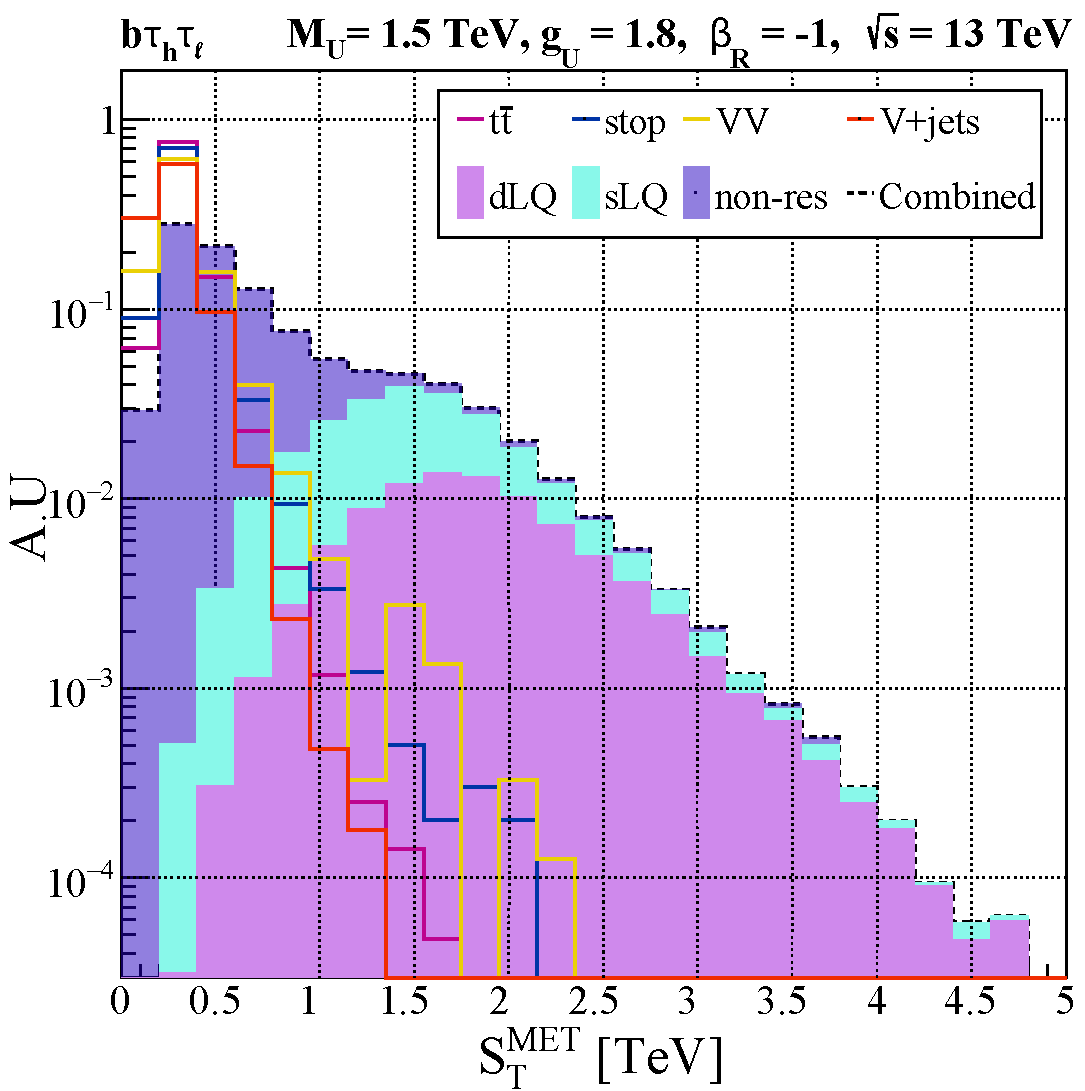
\includegraphics[width=\linewidth]{../Images/sTTeV_semileptonic_sLQ_wRHC.pdf}
		\end{block}
	\end{minipage}
	\hfill
	\begin{minipage}[t]{0.47\textwidth}
		\begin{block}{$\Delta R$ Separation}
		\vspace{-1.2em}
		\centering
		\[\Delta R = \sqrt{\Delta \eta^2 + \Delta \phi^2}\]
		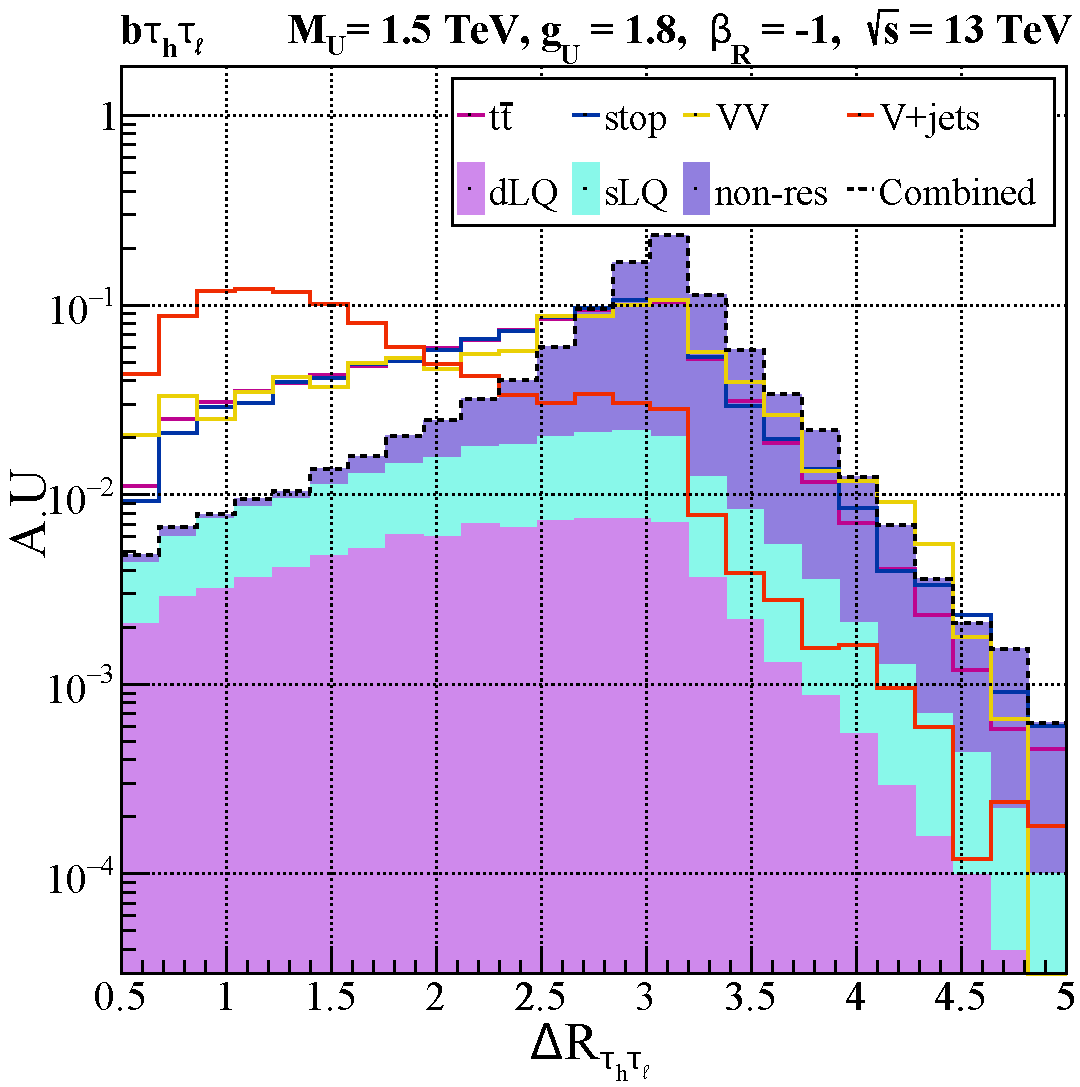
\includegraphics[width=\linewidth]{../Images/DeltaR_semileptonic_sLQ_wRHC.pdf}
		\end{block}
	\end{minipage}
	\vfill
	{\large
	\begin{itemize}
		\item Separation of sLQ and dLQ with the backgrounds enhanced via $S_T^{\text{MeT}}$, a measure of the boostedness of the event.
		\item Separation of non-resonant production with the backgrounds enhanced via $\Delta R$ between the $\tau$ candidates.
	\end{itemize}
	}
\end{frame}

\begin{frame}{XGB-output}
	\vspace{-1.6em}
	\begin{center}
		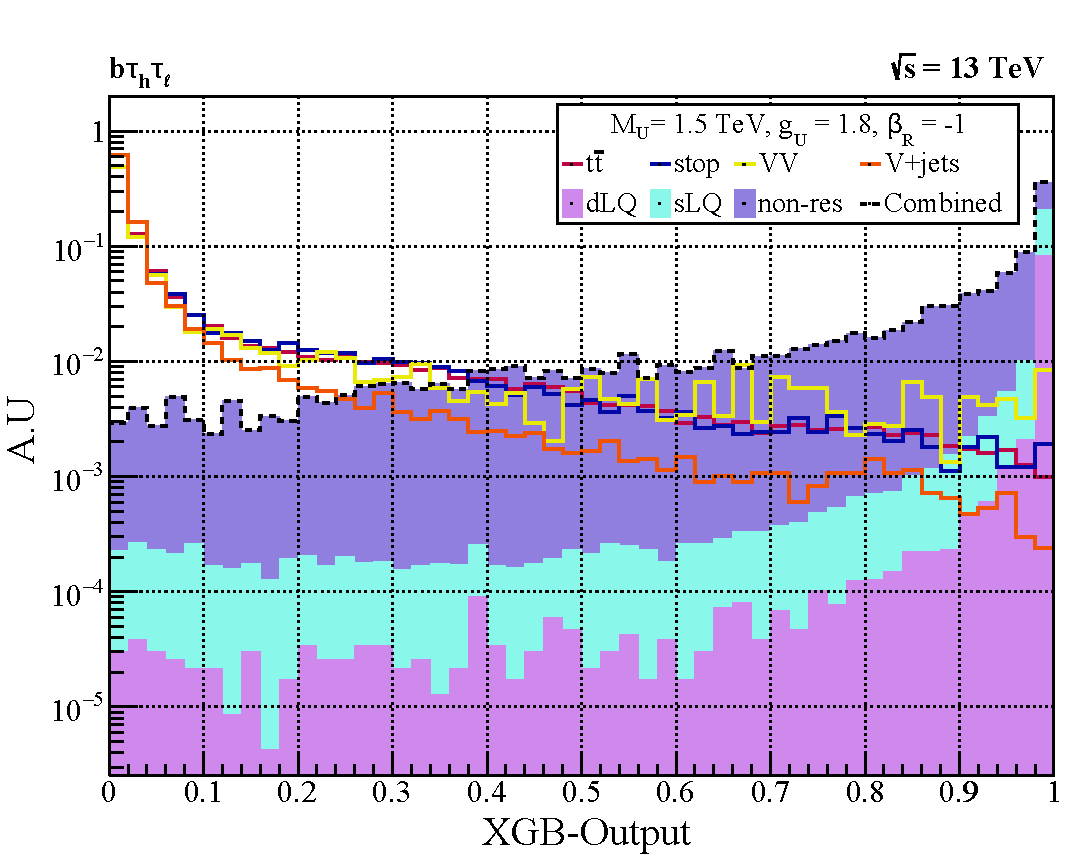
\includegraphics[width=.68\linewidth]{../Images/ML_semileptonic_sLQ_wRHC.pdf}
	\end{center}
	{\large
	\begin{itemize}
		\item We can evaluate a score for the signal and background events using the discriminator algorithm.
		\item Each production channel has contributions in each one of the six detection channels.
	\end{itemize}
	}
\end{frame}

\subsection{Single Channels Sensitivity Reach}

\begin{frame}{Double Leptoquark Production}{The Sensitivity Reach / only left-handed currents}
	\begin{minipage}{.30\linewidth}
		\includegraphics[width=\linewidth]{../Images/double_LQ.png}
	\end{minipage}
	\begin{minipage}{.68\linewidth}
		\includegraphics[width=\linewidth]{../Images/Significance_Heatmap_13TeV_L137_dLQ_combined_woRHC.pdf}
	\end{minipage}
	{\large
	\begin{itemize}
		\item dLQ production depends only on $\alpha_{\text{QCD}}$ and the available energy.
		\item So, the potential reach is independent of the global coupling with fermions $g_U$.
	\end{itemize}
	}
\end{frame}

\begin{frame}{Single leptoquark production}{The Sensitivity Reach / only left-handed currents}
	\begin{minipage}{.30\linewidth}
		\includegraphics[width=\linewidth]{../Images/single_LQ.png}
	\end{minipage}
	\begin{minipage}{.68\linewidth}
		\includegraphics[width=\linewidth]{../Images/Significance_Heatmap_13TeV_L137_sLQ_combined_woRHC.pdf}
	\end{minipage}
	{\large
		\begin{itemize}
			\item Single leptoquark production is sensitive to both, mass and couplings.
			\item It contributes to the regions of high coupling constants at higher masses than double leptoquark production.
		\end{itemize}
	}
\end{frame}

\begin{frame}{Non-resonant Production}{The Sensitivity Reach / only left-handed currents}
	\begin{minipage}{.30\linewidth}
		\includegraphics[width=\linewidth]{../Images/non_resonant.png}
	\end{minipage}
	\begin{minipage}{.68\linewidth}
		\includegraphics[width=\linewidth]{../Images/Significance_Heatmap_13TeV_L137_non-res_combined_woRHC.pdf}
	\end{minipage}
	{\large
	\begin{itemize}
		\item Non-resonant production is highly dependent on the couplings, so it dominates the regions of high coupling constants at all masses.
	\end{itemize}  
	}
\end{frame}

\subsection{Combined Sensitivity Reach}
\begin{frame}{Combined Sensitivity Reach}
	\begin{center}
		\includegraphics[width=.49\linewidth]{../Images/Significance_Curves_13TeV_L137_summary_all_sigmas_woRHC.pdf}
		\includegraphics[width=.49\linewidth]{../Images/Significance_Curves_Summary_by_BR.pdf}
	\end{center}
	{\large
	\begin{itemize}
		\item A combined analysis of the three production channels suggests better sensitivity for high coupling constants.
		\item Depending on the benchmark $\beta_L$, $\beta_R$ values, the branching ratio to $b \tau$ can vary, affecting the sensitivity reach.
	\end{itemize}
	}
\end{frame}

\begin{frame}{ATLAS Results}{Left-handed currents only}
	\begin{center}
		\includegraphics[width=.9\linewidth]{../Images/altas_lq.png}
	\end{center}
	{\large
	\begin{itemize}
		\item In parallel ATLAS relased a search following a similar approach [ArXiv:2305.15962]. 
	\end{itemize}
	}
\end{frame}

\begin{frame}
	\begin{center}
		\includegraphics[width=.8\linewidth]{../Images/Significance_Heatmap_13TeV_L137_all_combined_woRHC.pdf}
	\end{center}
	{\large
		\begin{itemize}
			\item Our ML-based analysis suggests better sensitivity for high coupling constants.
		\end{itemize}
	}
\end{frame}

\begin{frame}{Combined Sensitivity Reach}{The Sensitivity Reach / only right-handed currents}
	\begin{minipage}{.45\linewidth}
		\includegraphics[width=\linewidth]{../Images/cms_lq_excess.png}
	\end{minipage}
	\hfill
	\begin{minipage}{.53 \linewidth}
		\includegraphics[width=\linewidth]{../Images/Significance_CMS_Comparison_13TeV_L137_all_combined_woRHC.pdf}
	\end{minipage}
	{\large
		  The case $BR(lq \rightarrow b \tau) = 1$ corresponds to the only right-handed currents coupling. The sensitivity compared with the latest one from the CMS [2308.07826] and ATLAS Collaborations [2303.01294], again we suggest better sensitivity for high coupling constants.
	}
\end{frame}


\section{$Z'$ Interferences}

\ifsectiondividers
\begin{frame}
\centering
\vfill
{\Huge \textbf{$Z'$ Interferences}}
\vfill
\end{frame}
\fi

\begin{frame}{The need of a $Z'$ boson in gauge $U_1$ models}
    If $U_1$ has a gauge origin,  we could rewrite the interaction term in the covariant derivative as
	$$
	\psi_{L}^{\mathrm{SM}}=\begin{pmatrix}
		q_{Lr}\\ q_{Lg}\\ q_{Lb}\\ \ell_L
	\end{pmatrix}
	\Longrightarrow\;\;
	\mathcal{L}_{\text{int}}
	\sim U_{1\alpha}^\mu \bar{\psi}_{L}^{\mathrm{SM}}\, \gamma_{\mu} T_{+}^{\alpha } \psi_{L}^{\mathrm{SM}} + \text{h.c.},
	\quad
	T_{+}^{\alpha}=\begin{pmatrix}
		0 & 0 & 0 & \delta_{r\alpha}\\
		0 & 0 & 0 & \delta_{g\alpha}\\
		0 & 0 & 0 & \delta_{b\alpha}\\
		0 & 0 & 0 & 0
	\end{pmatrix},
	$$
	we have six generators $T_{\pm}^{\alpha }$ with closure relation and projecting into a color singlet operator:
	$$
	\sum_{\alpha} \left[{T_{+}^{\alpha }},{T_{-}^{\alpha}}\right] =
	3 T_{B-L}=\begin{pmatrix}
		1 & 0 & 0 & 0\\
		0 & 1 & 0 & 0\\
		0 & 0 & 1 & 0\\
		0 & 0 & 0 & -3
	\end{pmatrix}.
	$$
	So, the gauge group with this leptoquark must include a $U(1)_{B-L}$ symmetry (The right-handed currents also have a similar interaction term).
    
    \pause
    $$ $$
    The interaction terms for the $Z'$ boson have the form
	\begin{align*}
		\mathcal{L}_{\text{int}} &\sim Z'_\mu\left(\bar{\psi}_{L}^{\mathrm{SM}}\gamma^\mu (3T_{B-L}) \psi_{L}^{\mathrm{SM}}\right)\\
		&\sim Z'_\mu \left(\bar q_{L} \gamma^\mu q_{L} - 3 \bar \ell_L \gamma^\mu \ell_L\right).
	\end{align*}
\end{frame}
\begin{frame}{Interference with a $Z'$ vector boson}
\begin{minipage}{.48\linewidth}
	Non-Resonant Production (leptoquarks)
	\begin{center}
		\includegraphics[width=.9\linewidth,height=.5\linewidth]{../Images/non-res_vector.pdf}
	\end{center}
	\begin{equation}
		\mathcal{M}_{U_1} \sim \frac{1}{t-m_{U_1}^2 + i m_{U_1} \Gamma_{U_1}},
	\end{equation}
\end{minipage}
\hfill
\begin{minipage}{.48\linewidth}
	Resonant Production (neutral bosons)
	\begin{center}
		\includegraphics[width=.9\linewidth,height=.5\linewidth]{../Images/DY.pdf}
	\end{center}
	\begin{equation}
		\mathcal{M}_{Z'} \sim \frac{1}{s-m_{Z'}^2 + i m_{Z'} \Gamma_{Z'}},
	\end{equation}
\end{minipage}
so the interference has the form
	\begin{equation*}
		% \mathrm{RKI}
		% 			=\frac{1}{\sigma_{ LQ+Z'}}
					\dv{m}\left[
							\sigma_{ LQ+Z'}-\left(\sigma_{ LQ} +\sigma_{Z'}
							\vphantom{\frac{1}2}
							\right)
							\right]
							\sim \frac{g_{z'}g_{U}}{s}\frac{ m_{LQ}m_{Z'}\Gamma_{LQ}\Gamma_{Z'} - (t-m_{LQ}^2)(s-m_{Z'}^2)}{\left[
					(t-m_{LQ}^2)^2 + m_{LQ}^2\Gamma_{LQ}^2
			\right]
			\left[
					(s-m_{Z'}^2)^2 + m_{Z'}^2\Gamma_{Z'}^2
			\right]}.
	\end{equation*}

    Similary for Polarized final states.
\end{frame}

\begin{frame}{Interference with a $Z'$ vector boson}


	\begin{center}
		\includegraphics[width=.45\linewidth]{../Images/Kinematic_Interference_gu_1.0_gzp_1.0_zp_upper_limit_woRHC.pdf}
		\hfill
		\includegraphics[width=.53\linewidth]{../Images/xs_interference.png}
	\end{center}
\end{frame}

\begin{frame}{Effects on the Sensitivity reach}
	
	\begin{center}
		\includegraphics[width=.48\linewidth]{../Images/reach_wo_interference.png}
		\hfill
		\includegraphics[width=.48\linewidth]{../Images/reach_w_interference.png}
	\end{center}
	
\end{frame}

\begin{frame}
	\begin{center}
		\includegraphics[width=\linewidth]{../Images/lq_paper.png}
	\end{center}
\end{frame}

\section[Conclusions]{Summary and Conclusions}

\ifsectiondividers
\begin{frame}
\centering
\vfill
{\Huge \textbf{Summary and Conclusions}}
\vfill
\end{frame}
\fi

\begin{frame}

\end{frame}

\begin{frame}{Related Research Projects}
	\begin{center}
		\includegraphics[width=\linewidth]{../Images/scoto_paper.png}
		\pause\vfill
		\includegraphics[width=.9\linewidth]{../Images/ditaus_paper.png}
	\end{center}
\end{frame}

\begin{frame}{Future explorations}

	{\large
	\begin{itemize}
		\item We will explore the neutrino sector in the $U(1)_{T^3_R}$ model, including possible connections to dark matter, through a intensive study of the parameter space.
		\vfill
		\item Extended study of the $R(D)$, $R(D^*)$ anomalies in the context of the $U(1)_{T^3_R}$ model including right-handed neutrinos.
		\vfill
		\item We has been exploring models with new scalar doublets and singlets that exposes an alternative hypotesis for toponium-like psudoscalar resonance observed at the LHC.
		\vfill
		\item 
	\end{itemize}
	}
\end{frame}

\begin{frame}{Thank you for your attention!}
	% \begin{center}
	% 	\includegraphics[width=0.4\textwidth]{../Images/thank_you.png}
	% \end{center}
\end{frame}
%ADD a slide marker for backlog frames
\section{Backup}
\ifsectiondividers
	\begin{frame}
		\centering
		\vfill
		{\Huge \textbf{Backup Slides}}
		\vfill
	\end{frame}
\fi
\appendix

\begin{frame}{What Do We Look For at the LHC?}
	\vspace{-.4em}
    \begin{block}{Three Complementary Approaches}
        \begin{itemize}

            \item \textbf{SM Parameter Determination}
            \begin{itemize}
                \item Precisely measure fundamental SM parameters
                \item Test consistency of the SM framework
                \item Reduce theoretical uncertainties
            \end{itemize}

			\item \textbf{Indirect Searches (Precision Tests)}
            \begin{itemize}
                \item Measure SM processes with high precision
                \item Look for deviations in predicted distributions
                \item Constrain new physics through virtual effects
            \end{itemize}

            \item \textbf{Direct Searches}
            \begin{itemize}
                \item Look for new particles in final states (resonances, excesses)
                \item Examples: SUSY particles, $Z'$, leptoquarks, dark matter mediators
            \end{itemize}

        \end{itemize}
    \end{block}
    \vspace{-.4em}
    \begin{block}{Key Types of Measurements}
        \begin{minipage}{0.48\linewidth}
            \textbf{Direct Signatures:}
            \begin{itemize}
                \item Resonant mass peaks
                \item Excess events over SM background
                \item Missing transverse energy (MET)
                \item Unusual kinematic features
            \end{itemize}
        \end{minipage}
        \hfill
        \begin{minipage}{0.48\linewidth}
            \textbf{Precision Observables:}
            \begin{itemize}
                \item Differential cross sections
                \item Angular correlations
                \item Rare decay rates
                \item Lepton flavor universality ratios
                \item Charge-parity (CP) asymmetries
            \end{itemize}
        \end{minipage}
    \end{block}
\end{frame}

\section{Quark-Gluon Sea}
\begin{frame}{The Quark-Gluon Sea}
    
    \textbf{Partons} are the fundamental constituents inside protons: valence quarks (uud) and a \textbf{sea} of virtual quark-antiquark pairs and gluons.
    
    \begin{center}
        \includegraphics[width=\textwidth]{../Images/pp_collision.pdf}
    \end{center}

	The interacting partons are typically \textbf{sea quarks or gluons}, which carry only a fraction of the proton's momentum but dominate the cross-section at high energies.
\end{frame}

\begin{frame}{Jet Clustering \& Missing Transverse Momentum}
    \vspace{0.8em}
    
    \textbf{Jet clustering} groups collimated particle showers into jets to reconstruct the original quarks/gluons from the hard scatter.
    
    \vspace{1em}
    
    \textbf{Missing $p_T$} appears as transverse momentum imbalance, signaling undetected particles like neutrinos:
    \[
    \va*{p}_T^{\text{miss}} = -\sum_{\text{visible prods}} \va*{p}_T
    \]
	\begin{center}
        \includegraphics[width=0.90\linewidth]{../Images/real_event.png}
    \end{center}
    
\end{frame}




\section{FeynRules}
\begin{frame}{From Theory to Simulation: FeynRules}
	\begin{minipage}{0.60\textwidth}
        \centering
        \includegraphics[width=\textwidth]{../Images/Feynrules.png}
        \begin{block}{Why Simulate New Physics Models?}
            \footnotesize
            \begin{itemize}
                \item \textbf{Predict signals} for experimental searches
                \item \textbf{Test theoretical consistency} (unitarity, constraints)
                \item \textbf{Optimize analyses} before data collection
                \item \textbf{Interpret potential discoveries} from LHC data
                \item \textbf{Compare predictions} across different models
            \end{itemize}
        \end{block}
    \end{minipage}
	\hfill
    \begin{minipage}{0.35\textwidth}
        \begin{block}{Input: \texttt{.fr} Model File}
            \begin{itemize}\footnotesize
                \item Lagrangian $\mathcal{L}$ terms 
                \item Particle definitions: F, V, S fields
                \item Gauge symmetries: $SU(N)$, $U(1)$
                \item Parameters: masses, couplings
                \item Mixing matrices, constraints
            \end{itemize}
			\vspace{-0.3em}
        \end{block}
        
        \vspace{-0.5em}
        \begin{block}{Output: UFO Format}
            \begin{itemize}\footnotesize
                \item Complete Feynman rules (vertices)
                \item Lorentz and color structures
                \item Parameter definitions
                \item Ready to simulate
            \end{itemize}
			\vspace{-0.2em}
        \end{block}
        
        \vspace{-0.5em}
        
        \begin{block}{Features}
            \begin{itemize}\footnotesize
                \item[$\nearrow$] \textbf{Standardized} UFO format
                \item[$\nearrow$] \textbf{Flexible} for BSM models
                \item[$\nearrow$] \textbf{Community-driven}
                \item[$\searrow$] \textbf{NLO complexity}
                \item[$\searrow$] \textbf{Poor debugging}
                \item[$\searrow$] \textbf{Performance issues}
            \end{itemize}
			\vspace{-0.2em}
        \end{block}
    \end{minipage}
    
\end{frame}

\section{Hypothesis Testing \& Statistical Significance}
\begin{frame}{Statistical Significance}
    The statistical significance for discovery is a parametric test defined as:
    \begin{equation}
        \kappa = \frac{\Braket{t}_{B} - \Braket{t}_{S+B}}{\sigma_{S+B}}
    \end{equation}
    where $t = -2\ln[\mathcal{L}(n|S+B)/\mathcal{L}(n|B)]\sim \chi^2$ is the optimal test statistic.
	
	\vspace{1.0em}

	We denote $\mathcal{L}$ as the likelihood for Poisson-distributed event counts $n$ in each bin and gaussian systematic uncertainties.

	\vspace{1.0em}

    For binned data analysis, this simplifies to:
    \begin{equation}
        \kappa = \frac{\sum_i s_i w_i}{\sqrt{\sum_i (s_i + b_i + \delta_{\text{sys}}^2) w_i^2}}
    \end{equation}
    where $s_i$, $b_i$ are signal/background events in bin $i$, $w_i \sim \ln(1+s_i/b_i)$ are optimal weights, and $\delta_{\text{sys}}$ is the systematic uncertainty.

\end{frame}

\begin{frame}{Boosted Decision Trees vs Neural Networks}
	\begin{minipage}{.65\textwidth}
	\begin{center}
		\includegraphics[width=\textwidth]{../Images/BDTvsNN.jpg}
	\end{center}	
	\vspace{-1em}
			\begin{block}{BDTs}
			\textbf{Strengths:}
			\begin{itemize}\footnotesize
				\item \textbf{Interpretable}: Feature importance rankings
				\item \textbf{Robust}: Handle missing data well
				\item \textbf{Fast training}: Efficient on tabular data
				\item \textbf{Low hyperparameter tuning}: Reasonable defaults work
			\end{itemize}
			
			\textbf{Limitations:}
			\begin{itemize}\footnotesize
				\item \textbf{Extrapolation}: Poor outside training range
				\item \textbf{High-dimensional}: Can struggle with many features
				\item \textbf{Discontinuous}: Piecewise constant predictions
			\end{itemize}
		\end{block}
	\end{minipage}
	\hfill
	\begin{minipage}{0.32\textwidth}
		
		\begin{block}{Deep NNs}
			\textbf{Strengths:}
			\begin{itemize}\footnotesize
				\item \textbf{Flexible}: \\ Can learn complex non-linearities
				\item \textbf{High-dimensional}: \\Excel with many features
				\item \textbf{Continuous}: \\Smooth function approximations
				\item \textbf{Transfer learning}: \\Pretrained models possible
			\end{itemize}
			
			\textbf{Limitations:}
			\begin{itemize}\footnotesize
				\item \textbf{Black box}: \\Difficult to interpret
				\item \textbf{Data hungry}: \\Need large training sets
				\item \textbf{Computational}: \\Require GPUs for large networks
				\item \textbf{Sensitive}: \\Require careful hyperparameter tuning
			\end{itemize}
		\end{block}
		\vspace{-1em}
		\begin{block}{HEP Use Cases}
			\footnotesize
        	\textbf{BDTs}: 	Preferred for $\sim 10-100$ features \\
        	\textbf{NNs}: 	Preferred for low-level data (images, graphs)
		\end{block}
	\end{minipage}
	
\end{frame}



\begin{frame}{Feasible Experimental Signatures}{Kinematic Variables}
	\begin{figure}
	\centering
	\includegraphics[width=.6\linewidth]{../Images/PT_b1.pdf}
	\caption{Transverse momentum distribution of the leading \textrm{b}-quark jet candidate. The distributions are shown for the two main SM background processes and two signal benchmark points.\label{fig:pTb1}}
	\end{figure}
\end{frame}

\begin{frame}{Feasible Experimental Signatures}{Kinematic Variables}
	\begin{figure}
	\centering
	\includegraphics[width=.6\linewidth]{../Images/PT_mu1_1.pdf}
	\caption{Transverse momentum distribution of the leading muon candidate. The distributions are shown for the two main SM background processes and two signal benchmark points.\label{fig:pTmu1}}
	\end{figure}
\end{frame}

\section{Formalism of the gauge $U_1$ leptoquark}
\begin{frame}%{Formalism of the gauge $U_1$ leptoquark}
    Where the SM charges for the leptoquark, in the $Y=2(Q-T_3)$ convention, are
	\begin{center}
		\begin{tabular}{|c|c|c|c|c|}
			\hline & $\bar{q}_{L}$ & $\ell_{L}^{j}$ & $\bar{q}_{L}\gamma_{\mu} \ell_{L}$ & $U_{1}^{\mu}$ \\
			\hline$U(1)$ & $-1 / 3$ & $-1 $ & $-4 / 3$ & $+4 / 3$ \\
			\hline $\mathrm{SU}(2)$ & $\overline{\mathbf 2}$ & $\mathbf{2}$ & $\mathbf{1}$ & $\mathbf{1}$ \\
			\hline $\mathrm{SU}(3)$ & $\overline{\mathbf 3}$ & $\mathbf{1}$ & $\overline{\mathbf3}$ & $\mathbf{3}$ \\
			\hline
		\end{tabular}	
	\end{center}
	Then, the leptoquark $U_1 \sim \left(\mathbf{3}_{C}, \mathbf{1}_{I}, 4 / 3_{Y}\right)$. 

    \pause
    $$ $$
    The full Lagrangian for the vector leptoquark is
	\begin{align*}
		\mathcal{L}_{U}=&-\frac{1}{2} U_{\mu \nu}^{\dagger} U^{\mu \nu}+M_{U}^{2} U_{\mu}^{\dagger} U^{\mu}-i g_{s}U_{\mu}^{\dagger} T^{a} U_{\nu} G^{\mu \nu}_a -\frac{2 i}{3} g' U_{\mu}^{\dagger} U_{\nu} B^{\mu \nu}\\
		&+\frac{g_{U}}{\sqrt{2}}\left[U_{1}^{\mu}\left(\beta_{L}^{i j} \bar{q}_{L}^{i} \gamma_{\mu} e_{L}^{j}+\beta_{R}^{i j} \bar{d}_{R}^{i} \gamma_{\mu} e_{R}^{j}
		%+\beta_{N}^{i} \bar{u}_{R}^{i} \gamma_{\mu} N_{R}
		\right)+\text { h.c. }\right]
	\end{align*}
	where $U_{\mu \nu}=\mathcal D_{\mu} U_{\nu}-\mathcal D_{\nu} U_{\mu}$, $\mathcal D_{\mu}=\partial_{\mu}-i g_{s} G_{\mu}^{a} T^{a}-i \frac{2}{3} g_{Y} B_{\mu}$, and the couplings $\beta_{L}$ and $\beta_{R}$ are complex $3 \times 3$ matrices in flavor space. 

    \pause 
    $$ $$
    Constraints from $\Delta F=2$ and lepton flavor violation impose a hierarchy with dominant third generation couplings: 
    
    \begin{equation}
     \left|\beta_L^{11}\right|, \left|\beta_L^{12}\right|, \left|\beta_L^{21}\right|, \left|\beta_L^{22}\right|, \left|\beta_L^{31}\right| \ll \left|\beta_L^{13}\right| \ll\left|\beta_L^{23}\right|,\left|\beta_L^{32}\right| \ll\left|\beta_R^{33}\right|,\left|\beta_L^{33}\right|=\mathcal{O}(1)   ,
    \end{equation}
    where $\beta_R$ is diagonal.
\end{frame}

\section{Two body scattering}
\begin{frame}{Two body scattering}{CM-Frame}
    Consider the process
    \begin{equation}
        A(\va*{p}_1) + B(\va*{p}_2) \longrightarrow C(\va*{p}_3) + D(\va*{p}_4),
    \end{equation}
    \begin{center}
        \includegraphics[width=0.6\textwidth]{../Images/scatter.png}
    \end{center}

    From the Golden Rule, the cross section is given by
    \begin{equation}
        \sigma = \frac{n! (2\pi)^4}{4\sqrt{(\va*{p}_1\cdot\va*{p}_2)^2 - (m_1m_2)^2}}\int \abs{\mathcal{M}}^2\delta^{(4)}(p_1 + p_2 - p_3 - p_4)\frac{d^3\va*{p}_3}{(2\pi)^3 2E_3}\frac{d^3\va*{p}_4}{(2\pi)^3 2E_4}.
    \end{equation}
    But, in the CM frame, $\va*{p}_1 + \va*{p}_2 = 0$, where
    \begin{gather}
        \sqrt{(\va*{p}_1\cdot\va*{p}_2)^2 - (m_1m_2)^2} = E_1E_2 \abs{\va*{p}_1},
        \\
        \delta^{(4)}(p_1 + p_2 - p_3 - p_4) = \delta\left(
        E_1 + E_2 - E_3 - E_4
        \right)
        \delta^{(3)}(\va*{p}_3 + \va*{p}_4).
    \end{gather}
    Thus
    \begin{equation}
        \sigma = \left(\frac{1}{8\pi}\right)^2 \frac{n!}{(E_1E_2) \abs{\va*{p}_1}}\int \abs{\mathcal{M}}^2
        \frac{\delta\left(
            E_1 + E_2 - \sqrt{\va p_3^2 + m_3^2} - \sqrt{\va p_3^2 + m_4^2}
            \right)}{\sqrt{\va p_3^2 + m_3^2}\sqrt{\va p_3^2 + m_4^2}} \dd \va p_3
    \end{equation}
\end{frame}

\begin{frame}%{Two body scattering}{CM-Frame}
    Integrating over the radial part $\abs{\va p_3}$, we get
    \begin{equation}
        \sigma = \left(\frac{1}{8\pi}\right)^2 \frac{n! |\va*{p}_3|}{(E_1 +E_2)^2 \abs{\va*{p}_1}} \int \abs{\mathcal{M}}^2 \dd\Omega,
    \end{equation}
    with
    \begin{equation}
        |\va*{p}_3| = \frac{1}{2} \frac{\sqrt{((E_1+E_2)^2 - m_3^2 -m_4^2)^2- 4m^2_3m^2_4} }{E_1+E_2},
    \end{equation}
    the outgoing momentum in the CM frame.

    $$ $$

    We prefer work with differential cross section as
    \begin{equation}
        \frac{\dd \sigma}{\dd \Omega} = \frac{1}{64\pi^2} \frac{n! }{(E_1 +E_2)^2 } \frac{|\va*{p}_3|}{\abs{\va*{p}_1}} \abs{\mathcal{M}}^2.
    \end{equation}

    Defining $\sqrt s = E_1 + E_2$, we have
    \begin{equation}
        |\va*{p}_3| = \frac{1}{2} \frac{\sqrt{(s - m_3^2 -m_4^2)^2- 4m^2_3m^2_4} }{\sqrt s}, \quad  |\va*{p}_1|=\frac{1}{2} \frac{\sqrt{(s - m_1^2 -m_2^2)^2- 4m^2_1m^2_2} }{\sqrt s}.
    \end{equation}
    so the differential cross section is
    \begin{equation}
        \frac{\dd \sigma}{\dd \Omega} = \frac{1}{64\pi^2} \frac{n! }{s }
        \sqrt{\frac{(s - (m_3 + m_4)^2)(s - (m_3 - m_4)^2)}{(s - (m_1 + m_2)^2)(s - (m_1 - m_2)^2)}}
        \abs{\mathcal{M}}^2.
    \end{equation}

    Note that at this point, we don't need to know the explicit form of the matrix element $\mathcal{M}$, so it is a generic result.
\end{frame}

\begin{frame}{Writting $t$ in terms of $s$ and $\theta$}
    

    In general, there are three Lorentz-invariant useful kinematical variables to describe the scattering process, known as Mandelstam variables:
    \begin{align}
        \hat s & = (p_1 + p_2)^2 = (p_3 + p_4)^2 = m_1^2 + m_2^2 + 2p_1^\mu p_{2\mu }= m_3^2 + m_4^2 + 2p_3^\mu p_{4\mu}, \\
        \hat t & = (p_1 - p_3)^2 = (p_2 - p_4)^2= m_1^2 + m_3^2 - 2p_1^\mu p_{3\mu }= m_2^2 + m_4^2 - 2p_2^\mu p_{4\mu},  \\
        \hat u & = (p_1 - p_4)^2 = (p_2 - p_3)^2= m_1^2 + m_4^2 - 2p_1^\mu p_{4\mu }= m_2^2 + m_3^2 - 2p_2^\mu p_{3\mu}.
    \end{align}
    $$ $$
    In the CM-frame, $\hat s = s = (E_1+E_2)^2$. If, $m_3=m_4$ and $m_1=m_2$ with $E_1=E_2=E_3=E_4=E$, we have
    \begin{equation}
        t = -\left(\va p_1 - \va p_3\right)^2 = - \va p_1^2 - \va p_3^2 + 2\va p_1\va p_3 
    \end{equation}
    where $\va p_1^2 = E^2 - m_1^2 $  and $\va p_3^2 = E^2 - m_3^2 $.
    $$ $$
    So, in terms of $s$, $t$ could be written as
    \begin{equation}
        t= -2s + (m_1^2 + m_3^2) + 2\sqrt{(s/4 - m_1^2)(s/4 - m_3^2)} \cos\theta,
    \end{equation}
    with $\theta$ the scattering angle in the CM-frame.
\end{frame}



\end{document}
